\documentclass[10pt]{beamer}\usepackage[]{graphicx}\usepackage[]{color}
%% maxwidth is the original width if it is less than linewidth
%% otherwise use linewidth (to make sure the graphics do not exceed the margin)
\makeatletter
\def\maxwidth{ %
  \ifdim\Gin@nat@width>\linewidth
    \linewidth
  \else
    \Gin@nat@width
  \fi
}
\makeatother

\definecolor{fgcolor}{rgb}{0.345, 0.345, 0.345}
\newcommand{\hlnum}[1]{\textcolor[rgb]{0.686,0.059,0.569}{#1}}%
\newcommand{\hlstr}[1]{\textcolor[rgb]{0.192,0.494,0.8}{#1}}%
\newcommand{\hlcom}[1]{\textcolor[rgb]{0.678,0.584,0.686}{\textit{#1}}}%
\newcommand{\hlopt}[1]{\textcolor[rgb]{0,0,0}{#1}}%
\newcommand{\hlstd}[1]{\textcolor[rgb]{0.345,0.345,0.345}{#1}}%
\newcommand{\hlkwa}[1]{\textcolor[rgb]{0.161,0.373,0.58}{\textbf{#1}}}%
\newcommand{\hlkwb}[1]{\textcolor[rgb]{0.69,0.353,0.396}{#1}}%
\newcommand{\hlkwc}[1]{\textcolor[rgb]{0.333,0.667,0.333}{#1}}%
\newcommand{\hlkwd}[1]{\textcolor[rgb]{0.737,0.353,0.396}{\textbf{#1}}}%
\let\hlipl\hlkwb

\usepackage{framed}
\makeatletter
\newenvironment{kframe}{%
 \def\at@end@of@kframe{}%
 \ifinner\ifhmode%
  \def\at@end@of@kframe{\end{minipage}}%
  \begin{minipage}{\columnwidth}%
 \fi\fi%
 \def\FrameCommand##1{\hskip\@totalleftmargin \hskip-\fboxsep
 \colorbox{shadecolor}{##1}\hskip-\fboxsep
     % There is no \\@totalrightmargin, so:
     \hskip-\linewidth \hskip-\@totalleftmargin \hskip\columnwidth}%
 \MakeFramed {\advance\hsize-\width
   \@totalleftmargin\z@ \linewidth\hsize
   \@setminipage}}%
 {\par\unskip\endMakeFramed%
 \at@end@of@kframe}
\makeatother

\definecolor{shadecolor}{rgb}{.97, .97, .97}
\definecolor{messagecolor}{rgb}{0, 0, 0}
\definecolor{warningcolor}{rgb}{1, 0, 1}
\definecolor{errorcolor}{rgb}{1, 0, 0}
\newenvironment{knitrout}{}{} % an empty environment to be redefined in TeX

\usepackage{alltt}
\usepackage{amsmath}
\usepackage{amssymb}
\usepackage{geometry}
\usepackage{graphicx}
\usepackage{url}
\usepackage{bm}

\makeatletter
\let \@sverbatim \@verbatim
\def \@verbatim {\@sverbatim \verbatimplus}
{\catcode`'=13 \gdef \verbatimplus{\catcode`'=13 \chardef '=13 }} 
\makeatother
\IfFileExists{upquote.sty}{\usepackage{upquote}}{}
\begin{document}

% --------------------------------------------
\begin{frame}
\large
Lecture 14:\\ 
Multicollinearity\\
STAT 632, Spring 2020\\
\end{frame}

%--------------------------------------------
\begin{frame}{Multicollinearity}
When predictors in a regression model are strongly correlated there can be a number of issues:
\vspace{5pt}
\begin{itemize}
\item The signs of the coefficients can be the opposite of what we expect.
\vspace{5pt}
\item The standard errors are inflated so the t-tests may fail to reveal significant predictors.
\vspace{5pt}
\item The predictor variables are not significant when the overall F-test is highly significant.
\end{itemize}
\end{frame}

%--------------------------------------------
\begin{frame}{Multicollinearity}
Multicollinearity can be detected in several ways:
\vspace{5pt}
\begin{itemize}
\item Examining the relationships between the predictor variables in the scatter plot matrix.
\vspace{5pt}
\item Examining the correlation matrix of the predictor variables.
\vspace{5pt}
\item Variance inflation factors (VIFs).
\end{itemize}
\end{frame}

%--------------------------------------------
\begin{frame}{Variance Inflation Factor (VIF)}
Consider the multiple linear regression model with two predictors\\
$$Y = \beta_0 + \beta_1 x_1 + \beta_2 x_2 + e$$
\vspace{5pt}
It can be shown that
$$Var(\hat{\beta}_j) = \frac{1}{1-r^2_{12}} \cdot \frac{\sigma^2}{(n-1)S^2_{x_j}}$$
\begin{itemize}
\item $r_{12}$ denotes the correlation between $x_1$ and $x_2$\\
\item $S_{x_j}$ denotes the standard deviation of $x_j$
\end{itemize}
\vspace{5pt}
Notice that the variance of $\hat{\beta}_j$ increases as $r^2_{12}$ increases.  Thus, the correlation between the predictors increases the variance of the estimated regression coefficient.\\
% go over case with $r^2_{12} =0.99$ 
\end{frame}

%--------------------------------------------
\begin{frame}{Variance Inflation Factor (VIF)}
Consider the multiple linear regression model\\
$$Y = \beta_0 + \beta_1 x_1 + \beta_2 x_2 + \cdots + \beta_p x_p + e$$
It can be shown that
$$Var(\hat{\beta}_j) = \frac{1}{1-R_j^2} \cdot \frac{\sigma^2}{(n-1)S^2_{x_j}}$$
where $R^2_j$ is obtained from the regression of $x_j$ on all other predictors (i.e., the percent of variation in $x_j$ explained by the other predictors).\\
\vspace{10pt}
The term $\frac{1}{1-R_j^2}$ is called the \textbf{variance inflation factor} (VIF).  A commonly used rule is that a VIF greater than 5 indicates that there are issues with multicollinearity. 
\end{frame}

\begin{frame}{Variance Inflation Factor (VIF)}
For example, suppose that $R^2_j = 0.99$, then 
$$VIF_j = \frac{1}{1-0.99} = 100$$
The interpretation is that the standard error of the estimated regression coefficient, $se(\hat{\beta}_j)$, is $\sqrt{100} = 10$ times larger than it would be if there was no collinearity ($R^2_j=0$).
\end{frame}

\begin{frame}{Example\footnote{Example from Julian Faraway, \emph{Linear Models in R}, 1st edition, Ch. 5, pp. 83--87}}
\begin{itemize}
\item Car drivers like to adjust the seat position for their own comfort. Car designers would find it helpful to know where different drivers will position the seat depending on their size and age.
\vspace{5pt}
\item Researchers at the HuMoSim laboratory at the University of Michigan collected data on 38 drivers.
\vspace{5pt}
\item The response variable is \texttt{hipcenter}, the horizontal distance of the midpoint of the hips from a fixed location in the car in mm.
\vspace{5pt}
\item The predictors of interest are age, weight, height with and without shoes, seated height, arm length, thigh length, and lower leg length.
\end{itemize}
\end{frame}

%--------------------------------------------
% \begin{frame}
% \begin{figure}
% 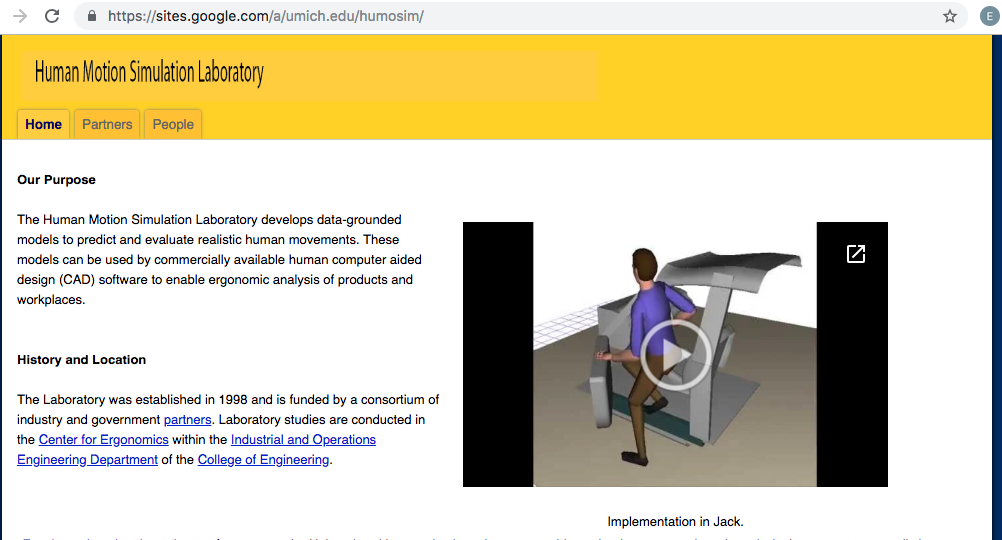
\includegraphics[scale=0.35]{figure/humosim}
% \end{figure}
% \end{frame}

%--------------------------------------------
\begin{frame}[fragile]
\small
\begin{verbatim}
> library(faraway)
> head(seatpos)
  Age Weight HtShoes    Ht Seated  Arm Thigh  Leg hipcenter
1  46    180   187.2 184.9   95.2 36.1  45.3 41.3  -206.300
2  31    175   167.5 165.5   83.8 32.9  36.5 35.9  -178.210
3  23    100   153.6 152.2   82.9 26.0  36.6 31.0   -71.673
4  19    185   190.3 187.4   97.3 37.4  44.1 41.0  -257.720
5  23    159   178.0 174.1   93.9 29.5  40.1 36.9  -173.230
6  47    170   178.7 177.0   92.4 36.0  43.2 37.4  -185.150
\end{verbatim}
\end{frame}

%--------------------------------------------
\begin{frame}
\begin{figure}
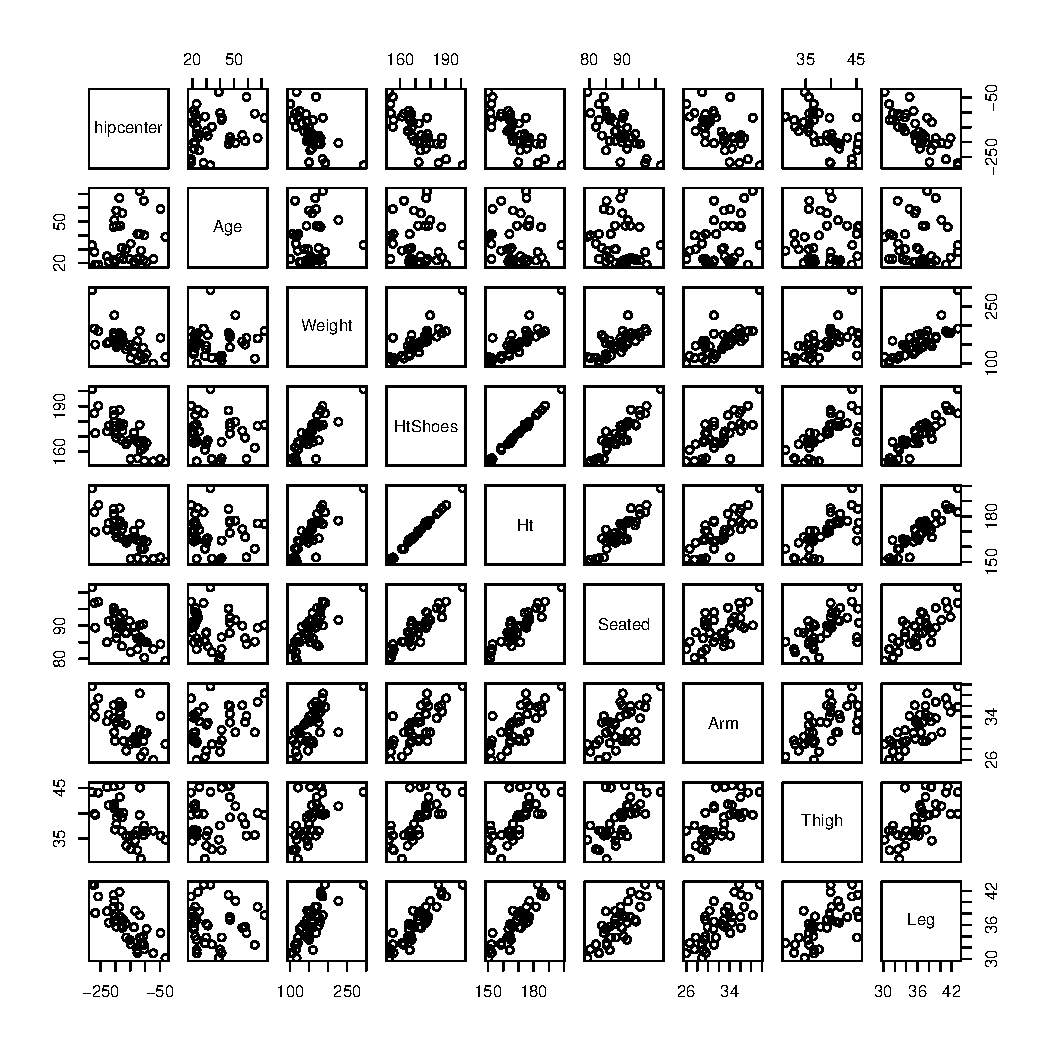
\includegraphics[scale=0.5]{figure/seatpos_pairs.pdf}
\end{figure}
\end{frame}

%--------------------------------------------
\begin{frame}[fragile]
There are several strong correlations between the predictors.
\small
\begin{verbatim}
> round(cor(seatpos[, -9]), 2)
          Age Weight HtShoes    Ht Seated  Arm Thigh   Leg
Age      1.00   0.08   -0.08 -0.09  -0.17 0.36  0.09 -0.04
Weight   0.08   1.00    0.83  0.83   0.78 0.70  0.57  0.78
HtShoes -0.08   0.83    1.00  1.00   0.93 0.75  0.72  0.91
Ht      -0.09   0.83    1.00  1.00   0.93 0.75  0.73  0.91
Seated  -0.17   0.78    0.93  0.93   1.00 0.63  0.61  0.81
Arm      0.36   0.70    0.75  0.75   0.63 1.00  0.67  0.75
Thigh    0.09   0.57    0.72  0.73   0.61 0.67  1.00  0.65
Leg     -0.04   0.78    0.91  0.91   0.81 0.75  0.65  1.00
\end{verbatim}
\end{frame}

%--------------------------------------------
\begin{frame}[fragile]
The model shows signs of multicollinearity.  The overall F statistic is large and $R^2=0.6$, but none of the individual predictors are significant.  
\scriptsize
\begin{verbatim}
> lm1 <- lm(hipcenter ~ ., data=seatpos)
> summary(lm1)
Coefficients:
             Estimate Std. Error t value Pr(>|t|)
(Intercept) 436.43213  166.57162   2.620   0.0138 *
Age           0.77572    0.57033   1.360   0.1843
Weight        0.02631    0.33097   0.080   0.9372
HtShoes      -2.69241    9.75304  -0.276   0.7845
Ht            0.60134   10.12987   0.059   0.9531
Seated        0.53375    3.76189   0.142   0.8882
Arm          -1.32807    3.90020  -0.341   0.7359
Thigh        -1.14312    2.66002  -0.430   0.6706
Leg          -6.43905    4.71386  -1.366   0.1824
---
Signif. codes:  0 ‘***’ 0.001 ‘**’ 0.01 ‘*’ 0.05 ‘.’ 0.1 ‘ ’ 1

Residual standard error: 37.72 on 29 degrees of freedom
Multiple R-squared:  0.6866,	Adjusted R-squared:  0.6001
F-statistic:  7.94 on 8 and 29 DF,  p-value: 1.306e-05
\end{verbatim}
\end{frame}

%--------------------------------------------
\begin{frame}[fragile]
Several of the variance inflation factors are large and exceed the 5 cut-off.\\
\small
\begin{verbatim}
> library(faraway) # to use vif() function
> round(vif(lm1), 2)
    Age  Weight HtShoes      Ht  Seated     Arm   Thigh     Leg 
   2.00    3.65  307.43  333.14    8.95    4.50    2.76    6.69 
\end{verbatim}
For \texttt{HtShoes} the interpretation is that the standard error for this predictor is $\sqrt{307.4} = 17.5$ times larger than it would be without collinearity.
\end{frame}

%--------------------------------------------
\begin{frame}[fragile]
We can also compute the VIFs manually.

\begin{verbatim}
# create data frame only containing predictors
> x <- seatpos[, -9] 

> summary(lm(Ht ~., data=x))$r.squared
[1] 0.9969982

> 1/(1 - 0.9969982)
[1] 333.1335
\end{verbatim}
\end{frame}

%--------------------------------------------
\begin{frame}{Your Turn}
\large
Manually compute the VIF for the predictor \texttt{Seated}, which is seated height in cm.\\
\end{frame}

\begin{frame}
\begin{itemize}
\item Many of the variables in the full model are redundant, and do the same job at predicting the response.
\vspace{5pt}
\item For example, the following predictors all measure the length of the driver in some way: \texttt{HtShoes}, height in shoes; \texttt{Ht}, height bare foot; \texttt{Seated}, seated height; \texttt{Arm}, arm length; \texttt{Thigh}, thigh length; and \texttt{Leg}, leg length.
\vspace{5pt}
\item Instead of using all of these length predictors, we can just select one to include in the model, and drop the others.
\vspace{5pt}
\item However, because of collinearity, we should not conclude that the variables we drop have nothing to do with the response.
\end{itemize}
\end{frame}

%--------------------------------------------
\begin{frame}[fragile]
Consider the correlation matrix with just the length variables.  All of these predictor variables are strongly correlated with each other.  We pick \texttt{Ht} since it is the simplest measure, and more strongly correlated with the response than the other predictors.
\small
\begin{verbatim}
> round(cor(seatpos[, 3:9]), 2)
          HtShoes    Ht Seated   Arm Thigh   Leg hipcenter
HtShoes      1.00  1.00   0.93  0.75  0.72  0.91     -0.80
Ht           1.00  1.00   0.93  0.75  0.73  0.91     -0.80
Seated       0.93  0.93   1.00  0.63  0.61  0.81     -0.73
Arm          0.75  0.75   0.63  1.00  0.67  0.75     -0.59
Thigh        0.72  0.73   0.61  0.67  1.00  0.65     -0.59
Leg          0.91  0.91   0.81  0.75  0.65  1.00     -0.79
hipcenter   -0.80 -0.80  -0.73 -0.59 -0.59 -0.79      1.00
\end{verbatim}
\end{frame}

%--------------------------------------------
\begin{frame}[fragile]
Removing some correlated predictors fixes many of the issues caused by multicollinearity.  The predictor \texttt{Ht} is now highly significant in the model.  Further simplification is clearly possible.\\
\scriptsize
\begin{verbatim}
> lm2 <- lm(hipcenter ~ Age + Weight + Ht, data=seatpos)
> summary(lm2)

Coefficients:
              Estimate Std. Error t value Pr(>|t|)    
(Intercept) 528.297729 135.312947   3.904 0.000426 ***
Age           0.519504   0.408039   1.273 0.211593    
Weight        0.004271   0.311720   0.014 0.989149    
Ht           -4.211905   0.999056  -4.216 0.000174 ***
---
Signif. codes:  0 ‘***’ 0.001 ‘**’ 0.01 ‘*’ 0.05 ‘.’ 0.1 ‘ ’ 1

Residual standard error: 36.49 on 34 degrees of freedom
Multiple R-squared:  0.6562,	Adjusted R-squared:  0.6258 
F-statistic: 21.63 on 3 and 34 DF,  p-value: 5.125e-08

> vif(lm2)
     Age   Weight       Ht 
1.093018 3.457681 3.463303 
\end{verbatim}
\end{frame}

\begin{frame}[fragile]
The $R^2$ of the reduced model with just 3 predictors (\texttt{Age}, \texttt{Weight}, and \texttt{Ht}) is close to the $R^2$ of the full model with all the strongly correlated predictors.  In fact, the adjusted $R^2$ for the reduced model is slightly higher than the full model.      
\begin{verbatim}
> summary(lm1)$r.squared
[1] 0.6865535
> summary(lm2)$r.squared
[1] 0.6561654

> summary(lm1)$adj.r.squared
[1] 0.6000855
> summary(lm2)$adj.r.squared
[1] 0.6258271
\end{verbatim}
\end{frame}

\begin{frame}{Concluding Remarks}
Some ways to deal with multicollinearity:
\vspace{5pt}
\begin{itemize}
\item If several predictors are strongly correlated with each other, pick one predictor out of the bunch to use in the reduced model.  The $R^2$ should not change much after removing some correlated predictors.
\vspace{5pt}
\item You can also combine predictors.  For instance, by taking the sum or average of two correlated predictors.
\vspace{5pt}
\item Automated variable selection techniques (e.g., stepwise selection, LASSO) can also be used (see ISLR, Ch.~6).
\end{itemize}
\end{frame}

% \begin{frame}{Concluding Remarks}
% \begin{itemize}
% \item Inspection of the correlation is not the only way to deal with multicollinearity and simplify the model.
% \item Stepwise variable selection methods can be used to reduce the number of predictors.
% \item Model techniques such as LASSO or ridge regression are also commonly used, and becoming increasingly popular (ISLR, Ch. 6).
% \item Hierarchical clustering is also a way to identify groups of correlated variables (ISLR, Ch. 10). 
% \end{itemize}
% \end{frame}


\end{document}
